\section{Flächen in Kartesische Koordinaten}

\begin{itemize}
	\item\textit{Eine Fläche S ist eine \textbf{Regelfläche} falls durch jeden ihrer Punkte eine Gerade existiert, die vollständig in S liegt.}
	\item\textit{\textbf{doppelte Regelfläche} falls durch jeden ihrer Punkte zwei unterschiedliche Geraden existieren}
\end{itemize}



\textbf{Explizite Darstellung} \\
\textit{Sattel:}
$z = f(x,y) = x^2 - y^2$ \\
\\
\textbf{Implizite Darstellung} \\
\textit{Kugel:}
$(x-x0)^2 + (y-y0)^2 + (z-z0)^2 = R^2$ \\
\textit{x0, y0, z0 = Zentrum}
\\
\textbf{Parameterdarstellung} \\

Zylinderkoordinaten:
\textit{$(r,\theta,z)$}
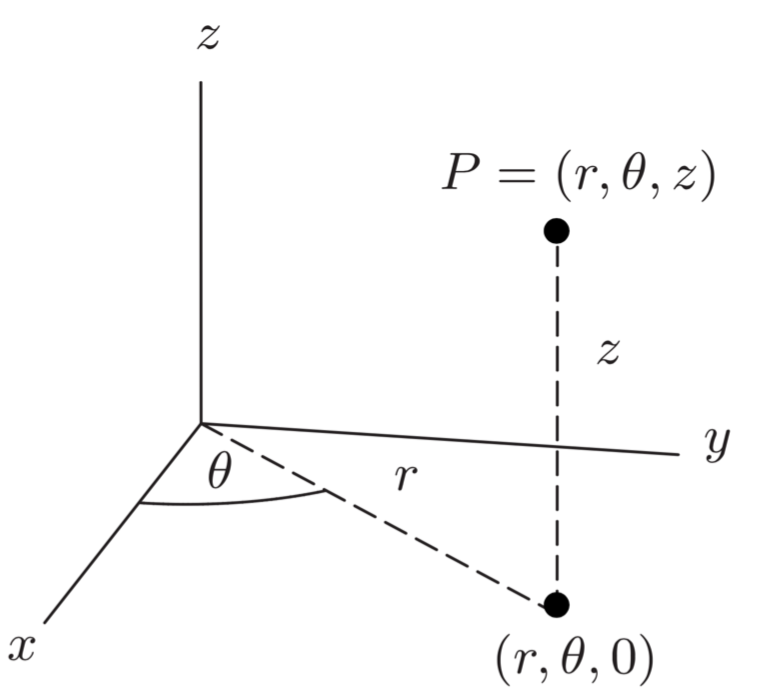
\includegraphics[width=0.3\textwidth]{assets/Zylinderkoordinaten.png}
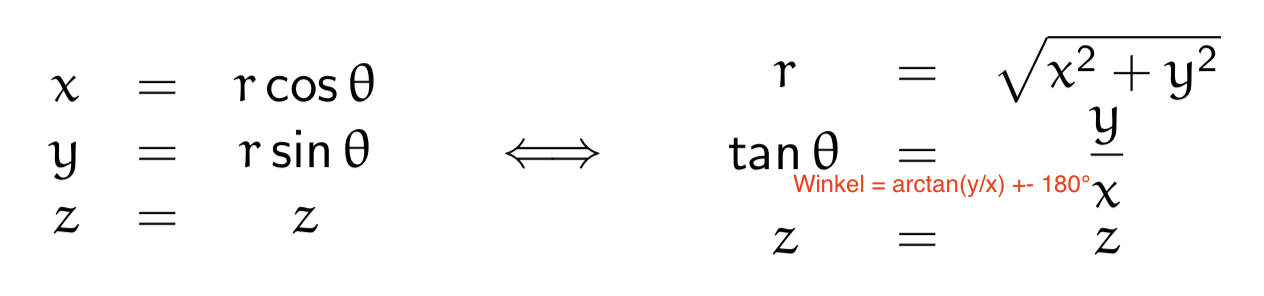
\includegraphics[width=0.3\textwidth]{assets/ZylinderkoordinatenUmrechnnung.png}

Kugelkoordinaten:
\textit{$(\rho,\phi,\theta)$}
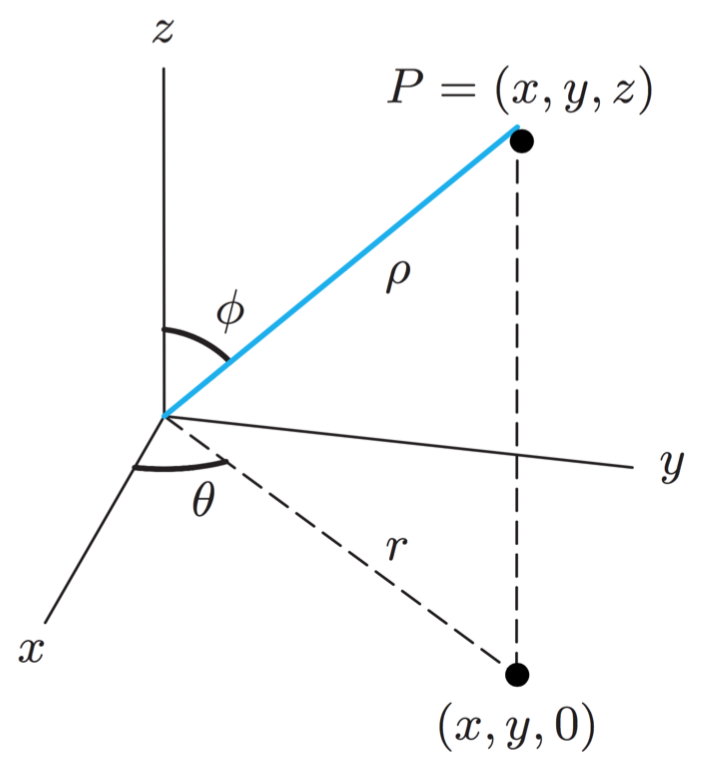
\includegraphics[width=0.3\textwidth]{assets/Kugelkoordinaten.png}
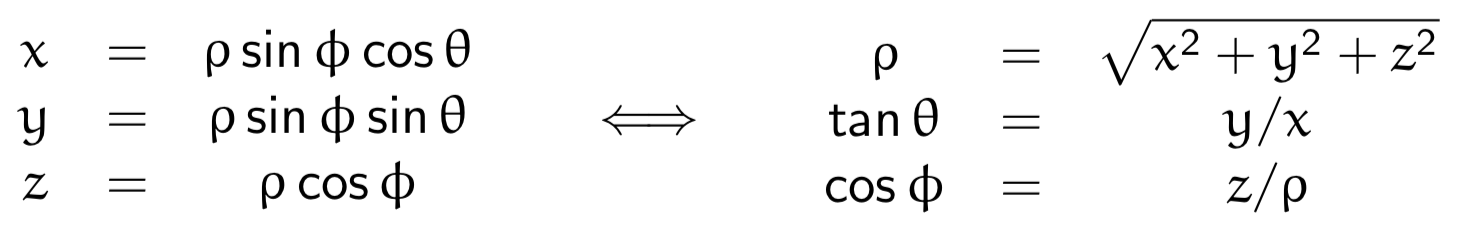
\includegraphics[width=0.3\textwidth]{assets/KugelkoordinatenUmrechnung.png}


Rotationsfläche:
\textit{$x=u$}
\textit{$y = f(x) * cos(v)$}
\textit{$z = f(x) * sin(v)$}
\subsection{Freiformflächen}
TODO

\begin{itemize}
	\item Tensorproduktfläche S(u,v) = Fläche gegeben von Kurven F(u) \& G(v) \\
	\textit{Für jeden u Wert gibt es eine Kurve -> "Gitterpunkte"}
\end{itemize}